\documentclass{article}
\usepackage[T1]{fontenc}
\usepackage{lmodern}
\usepackage{graphicx}
\usepackage{amsmath,amssymb}
\usepackage[a4paper,margin=2cm]{geometry}
\usepackage[absolute,overlay]{textpos}
\setlength{\TPHorizModule}{1mm}
\setlength{\TPVertModule}{1mm}
\usepackage[indonesian]{babel}
\usepackage{hyperref}
\setlength{\emergencystretch}{2em}
% unit: Halaman 18

\begin{document}

% === Halaman 18 (llm) ===

\vspace{154.44mm}

\section*{Program Caesar Cipher dalam Bahasa Python (256 karakter ASCII)}

% deskripsi: Screenshot potongan kode Python untuk fungsi enkripsi dan dekripsi Caesar Cipher menggunakan 256 karakter ASCII.
% bbox normalisasi: [0.0500, 0.2000, 0.9400, 0.7200]
\begin{textblock*}{186.90mm}(10.50mm,59.40mm)
\noindent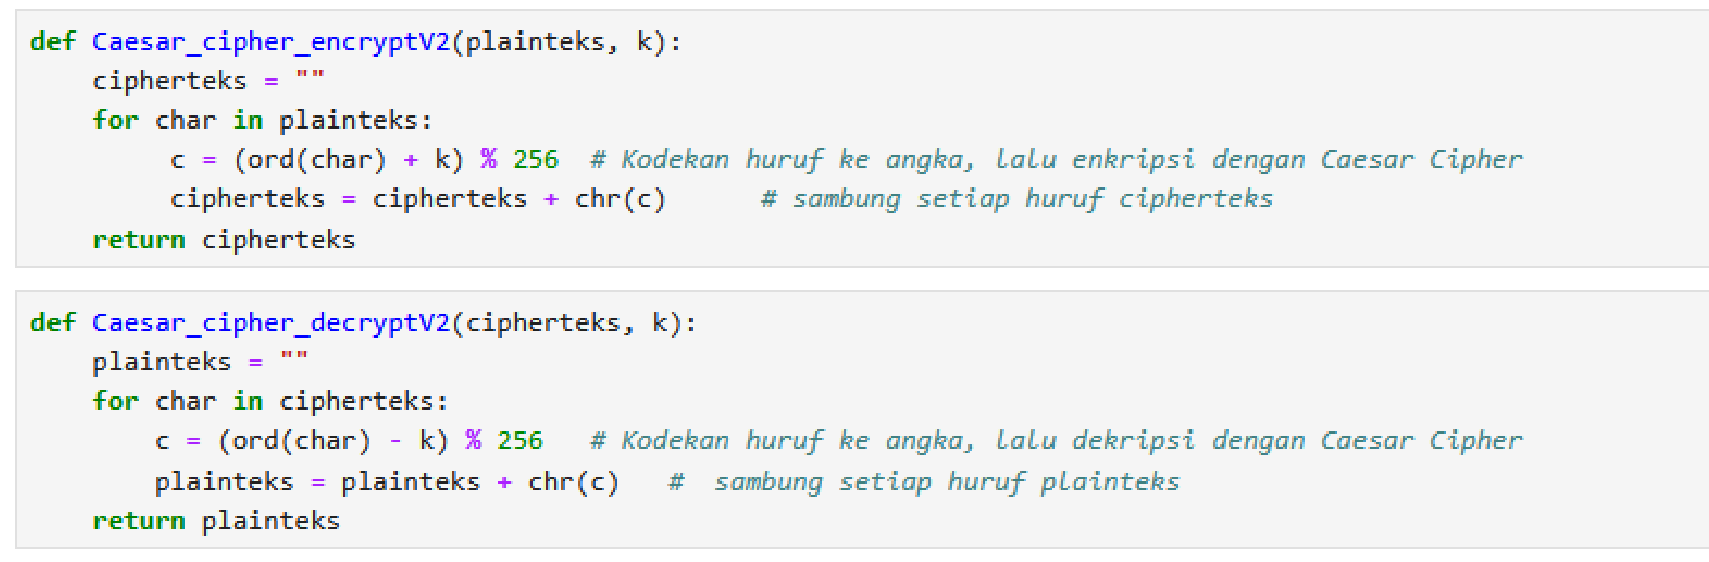
\includegraphics[width=186.90mm,height=154.44mm]{../../images/llm/page_018_img_01.png}%
\end{textblock*}

\end{document}
